\chapter{Write Away 10}

\begin{figure}[H]
    \centering
    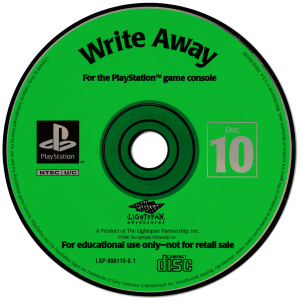
\includegraphics[width=\textwidth/2]{Games/WriteAway/Images/WriteAway10CD.png}
    \caption{Write Away 10 CD}
\end{figure}

The last of the ten Write Away games published and released by The Lightspan Partnership for the PlayStation 1.

Write Away 10 features ten video programs, including an introduction video, eight story videos, and a conclusion video:

\begin{itemize}
    \item Write Away Episode Ten Introduction
    \item The Sleigh Ride by Angela Dibella
    \item The Thing in the Gym by Jennifer Wisdon
    \item My Mom by Garrick Benally
    \item The Time Warp by Ashley Hudspeth
    \item The Young Man from Chile by Rogelio Ortega
    \item The Apple by Courtney Morris
    \item I Can't Wait to Play by Kristi Chitwood
    \item The Sea Monster in Elephant Butte by Vanessa Maesse
    \item Write Away Conclusion
\end{itemize}

\clearpage
\newpage

\section{Transcriptions}

\subsection{The Sleigh Ride by Angela Dibella}

SABRINA:
Here we are back at Write Away.
We have received some wonderful stories written by students like you from all across the nation.
Today is no exception.
It's amazing how with just two simple objects, a pencil and paper, your creativity has taken us all over the world, and introduced us to some very special people.
Our first story is a great example of how you can use your imagination to meet someone special, or travel to a place you've only ever imagined.
Our first author is Angela Dibella.
She's a second grader from Apalachee School in Tallahassee, Florida.
Come with us, as Angela takes us on an exciting sleigh ride.

ANGELA:
Hi everyone, here we are at the North Pole, the home of Santa Claus himself.
It's Christmas Eve, and I'm here to help Santa with all the presents he has to deliver.
Follow me.

MRS SANTA CLAUS:
And Bobby Jones from Minneapolis wants a football.

SANTA:
Check.

ANGELA:
Hi Santa.
Hi Mrs Claus.

SANTA:
Haha Angela, what are you doing up here at the North Pole?
And on the night before Christmas?

ANGELA:
I thought you could use some help, so here I am!

MRS SANTA CLAUS:
Oh we're so glad you're here, Angela.
The list of children that have been nice is extremely long this year.
We could really use your help.

ANGELA:
Well I'm ready.
What should we do first?

MRS SANTA CLAUS:
Let's make some hot cocoa.
Oh Santa always loves a cup of cocoa before he goes on one of his sleigh rides.

ANGELA:
Mmm...
It smells great.
Here's your coco Santa!

SANTA;
Well thank you Angela.
Mmm delicious.

ANGELA:
Well, what can I do now?

SANTA:
Would you please feed the reindeer for us?

ANGELA:
Oh I'd love to!

MRS SANTA CLAUS:
Right that way.

ANGELA:
You know Rudolph, your job is very important, because you light the way, so that Santa can see where all the houses are all over the world.

SANTA:
Hoho, very good.
Thanks to you Angela, I'm all ready to go.

ANGELA:
Santa, can I come with you and help you drive the sleigh?

SANTA:
Huhu, why of course!
Let's go.

ANGELA (VOICE OVER):
This was the best part of all.
I got to help Santa deliver presents to all the good little boys and girls.

ANGELA:
We've got a long ride ahead of us, so we better say goodbye for now.

SANTA:
Hohoho, Merry Christmas.

ANGELA:
The sleigh ride.
The end.

\subsection{The Thing in the Gym by Jennifer Wisdon}

JOE:
My favorite part of this job is reading all the scary stories that you've written for us.
Eugh.
You know, then kind of make your skin crawl and your spine tingle.
A good scary story has all the ingredients of suspense and mystery, and our next author has me holding on to my breath till the very, very end.
Jennifer Wisdom, a third grader from Central Elementary in Duncanville, Texas, has her characters clean everything up in 'The Thing in the Gym'.

PETER:
Yuh, my name is Peter, and I want to tell you a true story about the thing in the gym.
Well, people say that it's a ghost that lives in the gym, but I never believed them.
My Story begins.

PETER (VOICE OVER):
I was in the gym playing basketball with my friend when my tooth got accidentally knocked out.

GIRL 1:
Oh man, I'm sorry.

PETER:
Oh, it's okay, it's just my back tooth.
But there it is.

GIRL 1:
Wow!

PETER.
Here, I'll just stick it up here and I'll take it home later when I go home.

GIRL 1:
Okay, come on, let's keep playing!

PETER (VOICE OVER):
After play[ing], I forgot about my tooth and went home.

GIRL 1:
Augh man, look at the time.
I gotta go home.

PETER:
Yeah, me too.

GIRL 1:
Let's go.

PETER (VOICE OVER):
The next day when I went back to get my tooth, it was gone.
So I asked the janitor if he'd seen my tooth.

PETER:
Have you seen a tooth?

JANITOR:
A tooth you say?
No, I found a banana peel and some smelly gym socks and, and a lot of [that picture of Neil Sedaka].
But no tooth.
Ah, don't worry, son.
Your tooth will grow back.
Hey, maybe the thing in the gym took it.
Or maybe it was a ghost.

PETER:
I-I don't believe in ghosts.

JANITOR:
Well maybe and maybe not.
I gotta go clean the showers.
Later dude.

PETER (VOICE OVER):
Well, while the janitor was cleaning out the showers, something very weird happened.
Someone or something dropped a bottle of shampoo on the janitor's head.
Something was definitely going on.
So I decided to find out what it was, and got my sister Carrie to help.

PETER:
So, do we have all our supplies?

CARRIE:
Yes.
Stew for dinner, a camera, and the first aid kit, in case one of us gets attacked by that thing in the gym.

PETER:
Okay, let's go.

CARRIE:
I-I don't see anything, just some balloons and streamers for the dance tomorrow night.
Let's go home.

PETER:
No, no.
This is where all the mysterious accidents have occurred.
In the gym, and in the boy's shower room.
Come on.

CARRIE:
Well, I'm not going in there, pee-ew!

PETER:
Quiet!
I think I hear something.

PETER (VOICE OVER):
Suddenly, we heard popping sounds, and that's when we saw it.

PETER:
*panicked*
I'll get it, you take a picture!
Aah, take a picture!

CARRIE:
Okay!
I got it!
Let's go home!
*new scene*
I got it, I got it, I got the film development.

PETER:
Good, let me see it, let me see it.

CARRIE:
It's furry, with big teeth, and a mask on.
It's - it's...

PETER:
It's a raccoon!
You mean, a terrifying thing in the gym...
was just a raccoon?
That popping sound we heard was the raccoon popping the balloons from the dance.

CARRIE:
Yeah, and everyone knows raccoons like to steal things.
He probably took your tooth, and dumped the shampoo on the janitor's head.
Hey, hey, let's call the zoo and get them to come catch the raccoon and take care of him.

PETER:
Yeah, good idea.

PETER (VOICE OVER):
The next day, the Zookeeper met us at the gym.

ZOOKEEPER:
What's up?
You say you have a wild beast for the zoo?

PETER:
No, it's not a wild beast.

CARRIE:
It's a raccoon!

ZOOKEEPER:
What?
No man-eating, vicious, slobbering wild beast?

PETER, CARRIE:
No!

ZOOKEEPER:
Good.
Come on, let's go catch that raccoon.
Here little raccoon, come here.
    [Come here] little raccoon.

*whispering*
It's got your tooth.
Give it to me!
It's got lots of people's teeth!
Take [it]!
Take it!
And I've gotcha!
All right, now I'm gonna take you to the zoo and give you a nice new home.
Well, we gotta go, bye kids.
Thanks!

CARRIE:
Bye.

PETER (VOICE OVER):
Once the Zookeeper took the raccoon to the zoo, everything went back to normal.
Until weird things started happening in the...
Cafeteria!
The end!

\subsection{My Mom by Garrick Benally}

SCOUT:
Sometimes it's hard to know how to even start a story.
Well one way is to write about something, or someone you know very well.
Like let's say, for example, your dog Fido.
Woof, woof.
Or, your weird aunt Bertha.
Well, our next author gives us a peek at someone he knows very well.
Garrick Benally, a fifth grader from Ojo Amarillo School in Fruitland, New Mexico, introduces us to his favorite person in 'My Mom'.

BOY (VOICE OVER):
I was born in Shiprock, and when I was a baby, I saw my mom.
I heard her laugh.

MOM:
*laughing*

BOY (VOICE OVER):
Then we went home.
Soon I felt like a free baby.
When I grew a little older, I wished I could have a dog.
I think it was the best time of my life.

BOY:
And that's my mom!
The end.

\subsection{The Time Warp by Ashley Hudspeth}

JASMINE:
Writing is fun because you can create anything you want.
In just this past year, our young authors have created space aliens, monsters, time machines, and terrible villains.
It's always enjoyable for us to see what your imaginations have conceived.
I especially enjoy stories that give us a glimpse of a time long ago.
Ashley Hadspeth, a student at Booker T. Washington School in Mesa, Arizona, lets us see what might happen if we were caught up in a time warp.

NARRATOR (JENNIFER):
Once there was a boy named Tom who always played baseball with his friends Bob and Joe.

BOB:
Okay, you play outfield, Tom, because you're not very good at batting.

JOE:
Yeah, like you're really good at catching.

TOM:
Okay you guys.
Hehehe.

NARRATOR (JENNIFER):
Joe, hit the ball out to left field, and Tom yelled.

TOM:
I got it!
I got it!

NARRATOR (JENNIFER):
Suddenly, everything went dark.
When Tom woke up, he was no longer on the baseball field.
He was in a medieval castle.

TOM:
I got it, I got it!
I- oh- ooh where am I?
Oh, look at all these jewels.
Oh, and all this delicious food.
    [Told that] we're not in Kansas anymore.
I don't know where I am, but I better eat.

NARRATOR (JENNIFER):
Tom ate and ate until suddenly the wind blew a window open, and Tom looked outside to see a beautiful garden.

TOM:
This looks like my mom's garden.
But something's different.
I'm gonna investigate.
This isn't my mom's garden; this is the garden in a castle.
I must be in a time warp.

NARRATOR (JENNIFER):
Tom walked into the beautiful garden and started to get homesick, thinking about his mom.

TOM:
I miss my parents, and my home, and my friends.
How did I get here?
I don't know how to get back.
How did I travel back in time?
What year is it?

NARRATOR (JENNIFER):
Suddenly, a knight on horseback appeared, and Tom asked him.

TOM:
What year is it?

KNIGHT:
Why, it's 1522, and I bet you're wondering where you are, who am I, and how did you get here?
Sorry, can't tell you that.
No, my lips are sealed.
Hmm mmm mmm.
Mom's the word.
But if you were to happen to hear voices that were familiar to you, like let's say Joe and Bob and your mum, well, and you happen to go in the direction of where the voices came from, eh eh, ah then I suppose one might be able to find one's way home.
But... don't ask me.
What do I know?
I'm just a knight.
On a horse.
Goodbye!

JOE, BOB, MOM:
*faint voices*

TOM:
Joe?
Mom?
Bob?
I'm coming!
I'm coming!

JOE:
Tom!

TOM:
Mom, Bob, Joe.
I'm coming!
I'm coming!

JOE:
Tom, wake up!

TOM:
I'm back!
Bob, Joe, you don't believe what happened to me.
I was in a time warp, and I went to a castle, and there was a lot of delicious food there, and some nice jewels and- and a strange man on a horse who help me!
I think...

JOE:
Tom, like you, got hit on the head with a ball.

BOB:
Yeah, it was just a dream.

TOM:
But it was real!

JOE:
Yah.
Right.

BOB:
Quick [go for] around Tom.
Let's play ball.

JOE:
Yah.

BOB:
Come on, let's play ball.

TOM:
But this time I bat!

NARRATOR (JENNIFER):
And so Tom never told anyone else about his adventure in the time warp again.

\subsection{The Young Man from Chile by Rogelio Ortega}

PAUL:
Roses are red, violets don't stink, but if they are dirty, hose them down.
No, that doesn't work.
I know what will help: when writing, use the resources available to you.
Encyclopedias, dictionaries, a rhyming dictionary like this.
Got it!
Roses are red, violets don't stink, but if they are dirty, wash them in the sink.
Good!

You see when you use tools like this, they're a valuable resource that helps you put what's in your mind down on paper.
And whether or not our next writer used one of these, he has come up with a very amusing poem in the form of a limerick.
It was written by Rogelio Ortega, a fifth grader at Martin Luther King School in San Diego, California.
And he writes about a young man from Chile.

NARRATOR:
There was a young man from Chile, who had a new girlfriend named Millie.
They wanted to dance, and took time out to France, but they were showing off and being silly.
The Young Man from Chile.

\subsection{The Apple by Courtney Morris}

SABRINA:
Often writing involves a problem that needs to be resolved.
For example, if you take your character and put them up in a tree, then you have to get them back down.
Remember, a problem for your character doesn't have to seem important to you, only to him or her.
Courtney Morris is from Corpus Christi, Texas.
She's a first grader at Annaville Elementary.
Courtney tells us about her problem and how she solved it in her story entitled The Apple.

NARRATOR (JENNIFER):
Once our teacher got a red apple.

TEACHER:
Oh, thank you so much!
It's so shiny and red!

APPLE:
Hi there teacher.
You're looking pretty today.

TEACHER:
Oh ho, what a sweet Apple!
Oh, I'm not going to eat you.
I'm going to leave you here on my desk so I can look at you all the time!
I love you, you sweet little apple!

GIRL 1:
Teacher?

TEACHER:
What can't you see?
I'm talking to my Apple.

GIRL 2:
It's time to go home.

TEACHER:
Oh yes, good night everybody.
Good night, see you tomorrow.
Good night, good night.
Good night my sweet little apple.

APPLE:
Good night.

NARRATOR (JENNIFER):
That night, a worm got into our classroom.

WORM:
Let's see what's on this desk.
Ah, there's books, pencils, an eraser- and an apple?
An apple!

APPLE:
Oh no!

WORM:
Come here, you big juicy apple.
*eating the apple*
This is delicious.

NARRATOR (JENNIFER):
The next day, our teacher noticed the Apple was gone.

TEACHER:
Good morning students, now everyone open up your books to page...
Aah!
My apple is gone!

GIRL 2:
I think a worm ate it!
There's the core.

TEACHER:
Oh, my poor, sweet little apple!
You're gone!
What am I going to do without you?

NARRATOR (JENNIFER):
Our teacher cried all day long.
She cried so much, the classroom filled up with water.
The whole school could drown.

GIRL 2:
Oh, w-what should we do?

GIRL 1:
Oh, I know!
I've got another apple here in my lunch sack.
I'll give it to her, and maybe she'll stop crying.

NARRATOR (JENNIFER):
I gave her the Apple just in time.

TEACHER:
Oh thank you so much!
Oh, it looks just like my other sweet little apple.

APPLE:
Hi there teacher.

TEACHER:
I'm so happy!
No more school work today!
Let's party!

NARRATOR (JENNIFER):
So we all partied until we went home.
And we were all happy.

TEACHER:
Good night everybody, good night!
See you tomorrow.
Good night my sweet little apple.
I'll see you tomorrow too.

APPLE:
Good night.
*yawn*

\subsection{I Can't Wait to Play by Kristi Chitwood}

SCOUT:
Oh Joe, I can't wait, oh I can't wait!
I can't wait to do this next story!
It's gonna be so much fun!
Fun!

JOE:
Hahaha!
It's great when a writer can make the reader have just as much fun as they had in the story.
In fact, writing is all about sharing feelings and experiences.
The next experience our author shares with us is playing.
Kristi Chitwood, a second grader from J.J Izard Elementary in Van Buren, Arkansas, tires us out in her story 'I Can't Wait to Play'.

GIRL 1:
I can't wait to play, because I'm gonna have fun!
First, I'm gonna play with my friends.

GIRL 2:
You're it!

GIRL 1:
No, you're it!

GIRL 2:
No, you're it!

GIRL 1:
You're it!

GIRL 2:
You're it!

GIRL 1:
You're it!

GIRL 2:
You're it!

GIRL 1:
[Scram]
I'm gonna play with my cousin.
Come on, hopscotch!
My turn!
Go, faster, faster, faster!
Then I'm gonna play with my cat!

CAT:
Meow.

GIRL 1:
Then I'm gonna go play with my dog!
Okay, go fetch!
Quick, quick!
Fetch!
Fetch!
Then I'll play with my friend again!

GIRL 2:
You're it!

GIRL 1:
You're it!

GIRL 2:
You're it!

GIRL 1:
You're it!

GIRL 2:
You're it!

GIRL 1:
Then, I'll feed my fish.
Here, fishy fishy.
You want some more?
Take it all!
Then, I'll play with my Barbie.
Oh Barbie, you've been such a good girl.
I'm going to brush your hair and then you're going on a date with Ken!
Then, I'll play with my cat and my dog!

CAT:
Meow!

GIRL 1:
Go fetch!
Go fetch!

CAT:
Meow!

GIRL 1:
Hey, where is everybody?
Oh well, I can't wait till recess, because I'm gonna play again and I'm gonna have fun!

\subsection{The Sea Monster in Elephant Butte by Vanessa Maesse}

SCOUT:
Even in the strangest situations, lessons can be learned.
We're all familiar with Aesop's fables, where we're taught lessons through stories written about animals.
But this next story's not about a cute little rabbit, or a cuddly little squirrel.
It's about two boys in peril, and the lesson they learn is hammered home in a way that will keep you on the edge of your seats!
Woo hoo!
Vanessa Maesse, a third grader from Helen Ball Elementary in El Paso, Texas, teaches us a very valuable lesson in her horrific story entitled 'The Sea Monster from Elephant Butte'.

NARRATOR (JOE):
Submitted for your approval, the date: March 7th, 1993.
The place: a cold, foggy lake called Elephant Butte.
Two kids on an innocent fishing trip are about to have the adventure of their lives in 'The Scary Zone'.
Picture this: two kids, Jerry and Jason, fishing in the middle of Elephant Butte.
Their mother was on the shore making supper.
Jason, the oldest boy, was also known as a big brat.
He was always teasing his younger brother Jerry.

JASON:
Oh Jerry, what's that coming over here?
It's coming right towards you!
I-it's a shark!

JERRY:
Aaah!

JASON:
Hahaha!
Got you!

JERRY:
Knock it off Jason.

NARRATOR (JOE):
Finally, Jerry snagged a fish.

JERRY:
Oh ooh oh, I got one!
It must be a big one, because I can hardly reel it in.

JASON:
Oh that's too bad, are you a big wimp?
Hahaha.

JERRY:
No really!
I can't do it myself.

JASON:
Oh, let me help you.

NARRATOR (JOE):
It was getting harder and harder to reel it in.
The boys were getting scared.

JERRY:
Eugh, Jason, it's been an hour.
My hand hurts.

JASON:
Jerry, I don't think this is any ordinary fish.

JERRY:
*falls into the water*
Waaaah!

JASON:
Jerry?
Jerry, are you okay?
Jerry, answer me!
Oh no, mom's gonna be really mad when she finds out about this.
Jerry!

NARRATOR (JOE):
Jerry suddenly the boat was bumped.
Jason became very scared.
Then he saw it - scales skimming the top of the water.
Jason's boat was being pushed toward a waterfall.

JASON:
Oh no, I'm being pushed over a waterfall.
I'd better hold o-aaaah!

NARRATOR (JOE):
Jason swam to shore, found his mother.

JASON:
Mom, mom!
A big sea monster pulled Jerry into the water, and then it pushed my boat over the waterfall!

MOM:
Jason, were you teasing your brother again?
Now where is he?

JASON:
I don't know, Mom, really.

MOM:
We have to find Jerry!
Come on, we'll find out the truth.

JASON:
It is the truth mom!

MOM:
Jerry?

JASON:
Jerry?

MOM:
Jerry?

JERRY:
Jerry?
There he is, Mom.

MOM:
Oh, oh!
Son, speak to me!

JASON:
Wake up Jerry, wake up!

JERRY:
Jason, mom.
Aah!
What happened to me?
I get [pot] marks all over me.

JASON:
You've been by a sea monster, remember?

MOM:
Jason, there's no such thing as sea monsters!
Maybe it was a dog, or a hungry little fish.
Come on, let's get you to the doctor.

DOCTOR:
So you say you were fishing?

JASON:
Yeah, and he was bit by a big sea monster, right Jerry?

JERRY:
I don't remember.

DOCTOR:
Oh, these are pretty big bites.
The mammal that did this would have to have pretty big teeth.
Are you sure your brother didn't bite you?

JASON:
I didn't bite him, I didn't bite him!
Why won't anyone believe me?

DOCTOR:
Don't worry, you'll be better in no time.

NARRATOR (JOE):
Soon Jerry was back to his old self, but he never remembered what happened.

MOM:
Now let's try to sit down and have a normal dinner like a normal family - and keep your teeth to yourself.

JASON:
But it didn't happen.
You remember, don't you Jeremy (Jerry)?
You were bit by a big sea monster, remember?
Remember?

JERRY:
No.
What's for dinner?

MOM:
Fish!

JERRY:
Oh, this reminds me of someone, haha.

NARRATOR (JOE):
They never went fishing (in) Elephant Butte again after the attack.
And as for Jason, he was never a brat to Jerry again.
Because he'd entered 'The Scary Zone'.

\subsection{Write Away Conclusion}

JENNIFER:
We hope you've enjoyed our show today.
Your stories are finished and all put away.

JOE:
But we'll come again another day.

SCOUT:
The stories you've seen through music and mine,

SABRINA:
Can be written by you if you just take the time.

PAUL:
So pick up a pencil and paper you'll see.

EVERYONE:
The adventures and magic that writing sets free.
So Write Away!

\section{Credits}

Executive Producers: Gregg Baker, Deborah Brucher Wren, Michael Wren;
Directors: Gregg Baker, Robin LeValley;
Technical Director: Joseph S. Abreu;
Cast: Paul David, Scout Jackson, Joe Lopez, Jr., Sabrina Lu, Jennifer Shelton;
Writers: Deborah Brucher Wren, Robin LeValley;
Music: Rick Illes, Michael Wren;
Cameras: Steve Raines, Andy Hall, Richard Crow;
Special Costume Design: Dianne Brucher;
Production Coordinator: Layne Sterling;

\clearpage
\newpage

\section{Screenshots}

\begin{figure}[H]
    \centering
    \begin{subfigure}{0.45\textwidth}
        \centering
        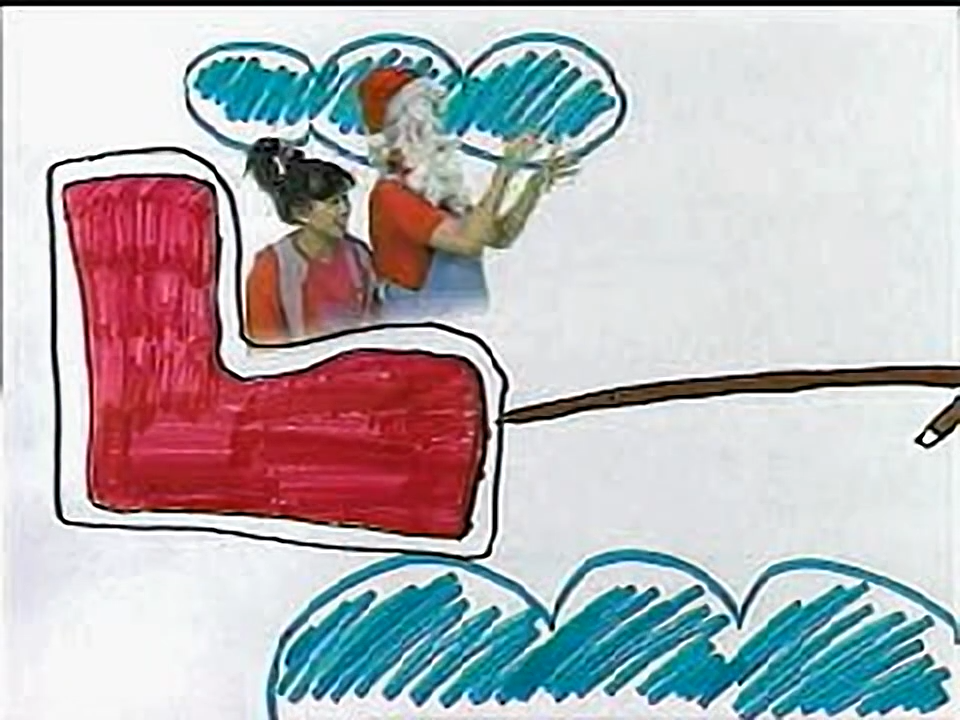
\includegraphics[width=\linewidth]{Games/WriteAway/Images/WriteAway10Screenshot1.png}
        \caption{Write Away 10 - Screenshot 1}
        \label{fig:sub1}
    \end{subfigure}
    \begin{subfigure}{0.45\textwidth}
        \centering
        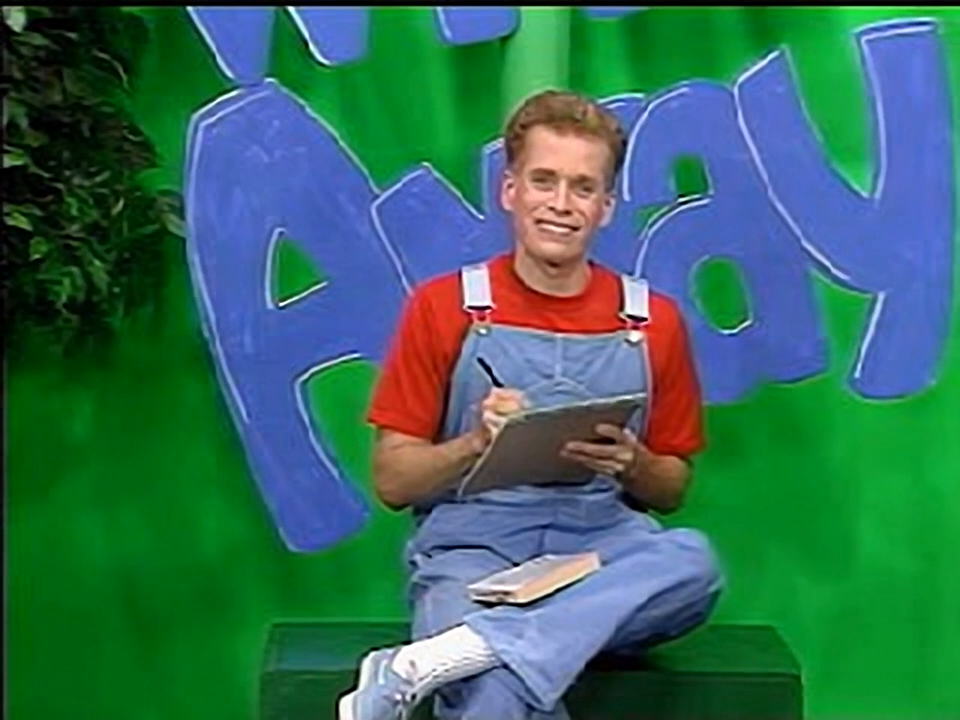
\includegraphics[width=\linewidth]{Games/WriteAway/Images/WriteAway10Screenshot2.png}
        \caption{Write Away 10 - Screenshot 2}
        \label{fig:sub2}
    \end{subfigure}

    \begin{subfigure}{0.45\textwidth}
        \centering
        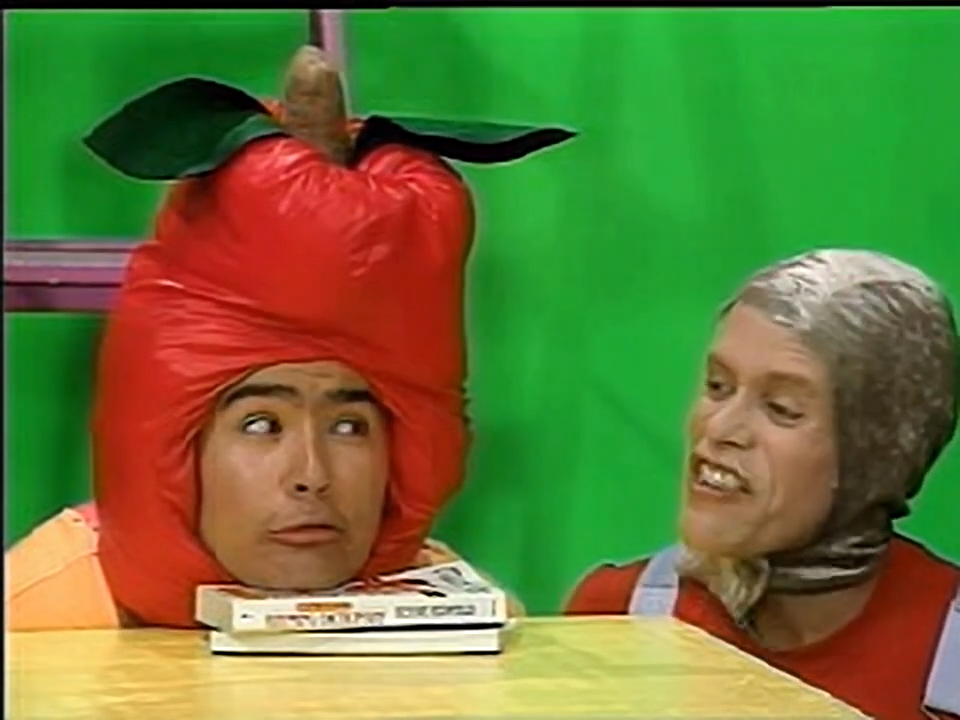
\includegraphics[width=\linewidth]{Games/WriteAway/Images/WriteAway10Screenshot3.png}
        \caption{Write Away 10 - Screenshot 3}
        \label{fig:sub3}
    \end{subfigure}
    \begin{subfigure}{0.45\textwidth}
        \centering
        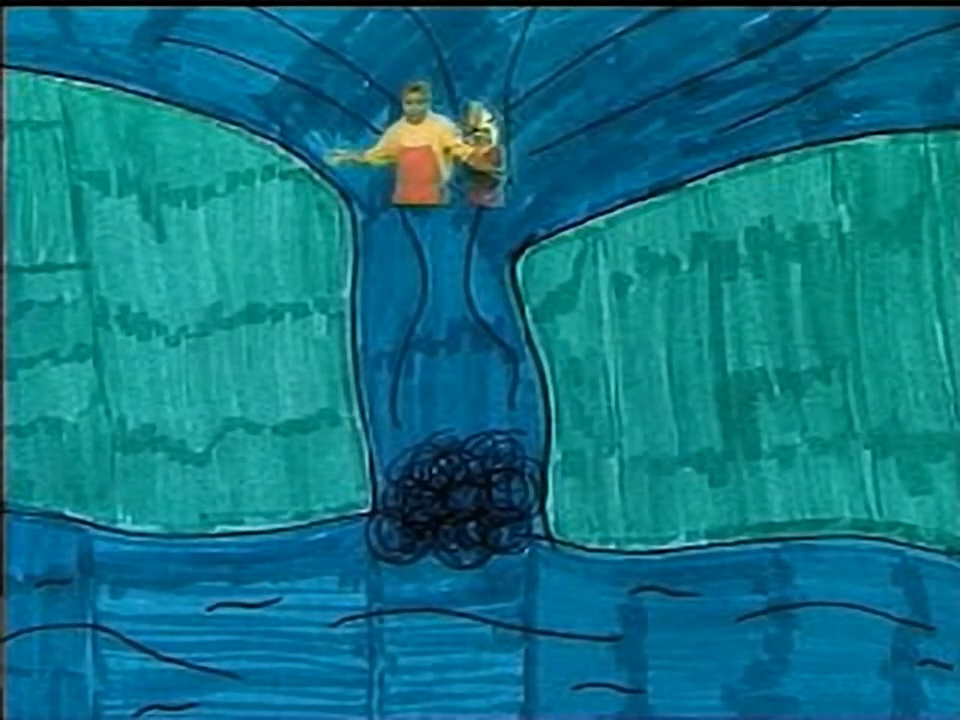
\includegraphics[width=\linewidth]{Games/WriteAway/Images/WriteAway10Screenshot4.png}
        \caption{Write Away 10 - Screenshot 4}
        \label{fig:sub4}
    \end{subfigure}
    \caption{Screenshots from Write Away 10}
    \label{fig:all}
\end{figure}
